%% ----------------------------------------------------------------
%% Background.tex
%% ---------------------------------------------------------------- 
\chapter{Theoretical Background} \label{Chapter:Background}

\section{Machine Learning}

Machine learning focuses on developing algorithms and models that enable computers to learn patterns from data and make predictions or decisions without being explicitly programmed for the task \cite{Murphy}. 
The use of statistical techniques such as linear regression allows it to improve its performance over time as it is exposed to more information. 
There are three commonly used machine learning approaches \cite{Bishop} including supervised learning, where the algorithm is trained on labeled data; 
unsupervised learning, where the algorithm discovers patterns in unlabeled data; and reinforcement learning, where the algorithms learn through trial and error based on feedback from its actions.

\subsection{Performance Measure}

In both machine learning and deep learning, the cost function is often the target to minimize. This function measures how well a model is performing on the training data.
In this project, mean squared error (MSE) and mean absolute percentage error (MAPE) have been considered. The functions of the two indicators are shown below:

\begin{gather}
    \mathrm{MSE} = \frac{1}{n}\sum_{i=1}^{n}(\hat{y_i} -y_i)^2 
\end{gather}

MSE calculates the square of the difference between the predicted value $\hat{y_i}$ and the actual value $y_i$, and takes the mean of it \cite{Bishop}. 
The value is in the range of $[0, +\infty)$, when the predicted value equals the real value, MSE is 0. As the difference gets larger, MSE increases. 

\begin{gather}
    \mathrm{MAPE} = \frac{100\%}{n} \sum_{i=1}^{n} \left | \frac{\hat{y_i}-y_i}{y_i} \right | 
\end{gather}

Instead of the actual value of the loss, MAPE is more focused on percentage \cite{Hyndman}. The range of MAPE is also $[0, +\infty)$, where a 0\% MAPE means a perfect match, and above 100\% would be considered as bad. 
Note that when the real value is in the denominator, which means it is not useable for any data set that contains a real value of 0.

\subsection{Gradient Descent}

Gradient descent is an optimization algorithm used to minimize the cost function iteratively. The gradient or derivative of the cost function at a point tells the direction of the steepest increase of the function. 
Hence if the parameters are updated in the opposite direction of the gradient, the model will be closer, and potentially reach the mimimum cost. 
The size of the the step of each update is controlled by the learning rate. 

For example in linear regression, we shell fit the data using a polynomial function \cite{Bishop}: 

\begin{gather}
    \hat{y}(x, \mathbf{w}) = \omega _0 + \omega _1x^1 + \omega _2x^2 + \dots +\omega _nx^n = \sum_{i=0}^{n}\omega _ix^i 
\end{gather}

Where the function has an order of n, with parameters $\omega_i$ controlling each term. These parameters are also denoted as vector $\mathbf{w}$ for future convenience.

The cost function using MSE hence can be denoted as:

\begin{gather}
    \mathrm{MSE} = \frac{1}{n}\sum_{i=1}^{n}(\hat{y}(x_i, \mathbf{w}) - y_i)^2 
\end{gather}

A step of gradient descent can be represented as below, repeat the process until achieving a certain level of accuracy, or other convergence criteria. 

\begin{gather}
    \mathbf{w}_{new} = \mathbf{w}_{old} - \alpha \times \nabla(\mathrm{MSE})
\end{gather}

\subsection{One-hot Encoding}

Sometimes the data used in machine learning contains categorical variables, which represent categories or labels, such as colors and the class of a road.
Each value of these variables is independent, the size does not matter. To let the model understand this better, one-hot encoding could be introduced.

One-hot encoding is a technique used to represent those categorical variables as binary vectors. The length of the vectors is equal to the number of unique categories,
and each position in the vector corresponds to a specific category. If the data is in a category, the corresponding position is set to be 1, otherwise, fill with 0. 
With this implemented, each category is treated as an independent entity and does not impose any ordinal relationship. 

\section{Deep Learning}

Deep learning is a subset of machine learning, which includes the use of neural networks. It is designed to solve complex problems with large datasets. 
Popular deep learning architectures include convolutional neural networks (CNNs), recurrent neural networks (RNNs), and transformers.

\subsection{Neural Network}

At the core of deep learning are artificial neural networks (ANN), which are inspired by the structure and functioning of the human brain. 
The structure of a neural network is illustrated in \fref{Figure:ANN-structure}. It is composed of layers of interconnected nodes (neurons). 
The input layer is where the data is fed into the network, and the output layer produces the final result. Between the input and output layers, there are one or more hidden layers 
each node in the hidden layers has a usually non-linear activation function. Section \ref{Section:activation} talks more about them. Lines between layers are linear transformations, 
with the parameter vector $\mathbf{w}$, and bias $\mathrm{b}$. 

\begin{figure}[!htb]
    \centering
    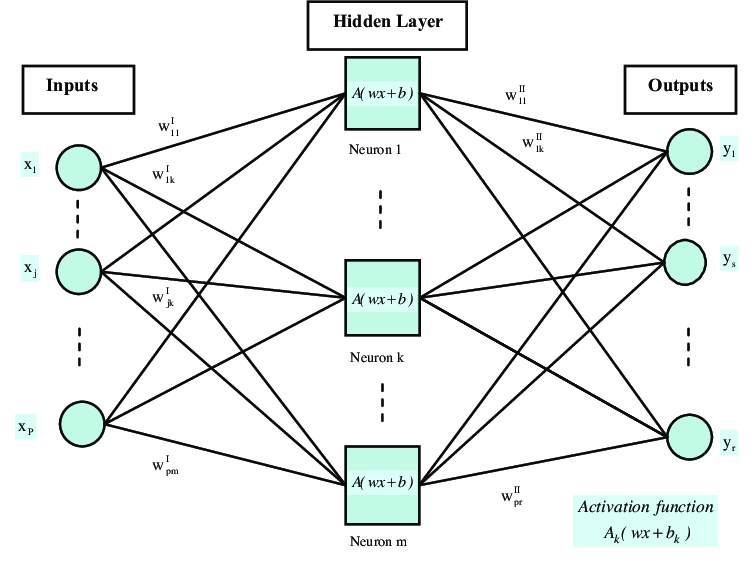
\includegraphics[width=12cm]{ANN-structure}
    \caption{A simple ANN structure with one hidden layer (Adapted from \cite{Kocadağlı})}
    \label{Figure:ANN-structure}
\end{figure}

What the network trying to do is the same as machine learning: find a function that best fits the data, so it can make predictions. The process could be expressed as:

\begin{gather}
    \mathbf{y} =\mathbf{w}^{II} \times A_k (\mathbf{w^Ix} + b^I_k)+ b^{II}
\end{gather}

The inputs fed into the network first go through a linear transformation and then map to an activation function. At last, go through a linear transformation again and output. 
By altering the parameters, it is possible to construct any curve. 

Deep learning emphasizes the use of deep neural networks, which means networks with multiple hidden layers. These networks are capable of learning complex datasets with non-intuitive 
characteristics. The depth allows the network to automatically learn features at different levels of abstraction.

Backpropagation is a key used in training deep neural networks. It is a supervised learning algorithm that adjusts the parameters $\mathbf{w}$
by propagating the error backward from the output layer to the input layer. This allows the network to update parameters to optimize predictions. 
Gradient descent is one of the backpropagation methods. Knowing the error from prediction, it measures which connection in the hidden layer.

\subsection{Activation Functions} \label{Section:activation}

The choice of activation function is vital in neural networks by introducing non-linearity into the model \cite{activation}. 
It enables the network to learn complex patterns and relationships in the data. 

\subsubsection{Rectified Linear Unit (ReLU)}

ReLU is one of the most commonly used activation functions. It replaces all negative values in the inputs with zero, which can be represented by: 
\begin{gather}
    f(x) = \mathrm{max}(0, x) 
\end{gather}

During the training, it will not activate all neurons at the same time, which gives an advantage that it is computationally efficient.
However, when $x < 0$, the gradient is zero. As training progresses, neurons may become inactive and weights fail to update.
To solve this problem, a variant of ReLU, Leaky ReLU, could be used instead. Leaky ReLU allows a small, non-zero gradient when the input is negative.

\begin{gather}
    f(x) = \mathrm{max}(\alpha x, x) 
\end{gather}

Where $\alpha$ is a small positive constant. A plot of both functions is shown in \fref{Figure:ReLUplots}

\begin{figure}[!htb]
    \centering
    \subcaptionbox{ReLU}{
        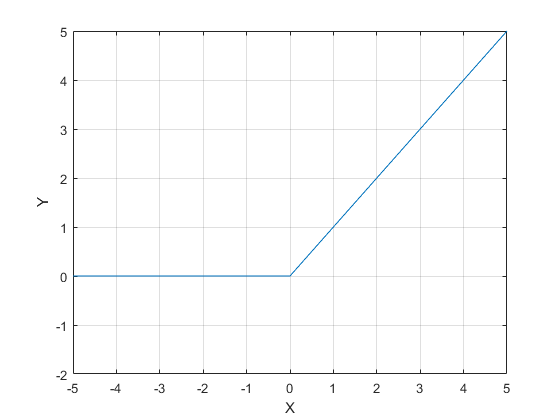
\includegraphics[width=6.5cm]{ReLU}
        \label{Figure:ReLUplots:ReLU}
    }
    \subcaptionbox{Leaky ReLU}{
        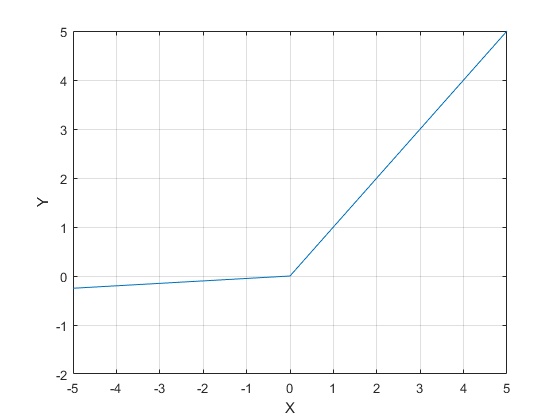
\includegraphics[width=6.5cm]{LeakyReLU}
        \label{Figure:ReLUplots:LeakyReLU}
    }
    \caption{ReLU activation functions}
    \label{Figure:ReLUplots}
\end{figure}

It is also possible to use the exponential linear units (ELU) to address the problem of inactive neurons. 
It uses $e^x-1$, which gives a similar curve, but has a small negative value at $x < 0$. 

\subsubsection{Other Functions}

There are many other activation functions such as sigmoid, hyperbolic tangent (Tanh), Softmax, etc.
Those are suitable for different purposes. For example, sigmoid have a limited output range, suitable to use before output. 
However, the curve gets too smooth at two ends, which causes a low learning efficiency. It is more used in classification problems. 

\section{Recurrent Neural Networks (RNNs)}

RNNs are a type of ANN designed for sequence data where the order of the data points is crucial \cite{lipton2015critical}. 
This makes RNN a good approach for this project. Similar to the simple ANN, RNN is constructed by multiple RNN cells. The formula of each cell is given by:

\begin{gather}
    \mathbf{h}_t = A (\mathbf{w^Ix}_t + \mathbf{w^{II}h}_{t-1} + b)
\end{gather}

Where $\mathbf{x}_t$ is the input at time $t$, $\mathbf{h}_t$ is the output at $t$, hence, $\mathbf{h}_{t-1}$ is the output at time $t-1$. 
Everything else is the same as the simple ANN. The essence of RNN is that the output of the current moment will take place in the calculation 
of the next moment as one of the inputs. \fref{Figure:RNN-structure} illustrates the idea of RNN.

\begin{figure}[!htb]
    \centering
    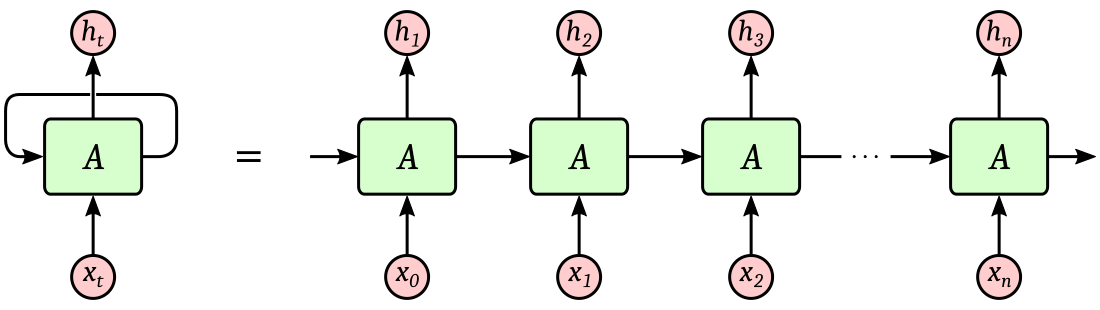
\includegraphics[width=12cm]{rnn}
    \caption{RNN as a neural network very deep in time (Adapted from \cite{rnnplot})}
    \label{Figure:RNN-structure}
\end{figure}

RNNs are susceptible to the vanishing/exploding gradient problem \cite{ribeiro2020exploding}. 
Since the RNN uses the backpropagation to minimize the cost function, and the error has been calculated from outputs going back through the network to update the weights, 
those weights in the feedback loop ($\mathbf{w_{rec}}$) are multiplied a lot of times during the backpropagation. 
If $\mathbf{w_{rec}} < 1$, the gradient will be vanishing, since it approaches 0. In contrast, If $\mathbf{w_{rec}} > 1$, then the weight will tend to be very large, i.e. exploding. 

\section{Long Short-Term Memory (LSTM)}

\begin{figure}[!htb]
    \centering
    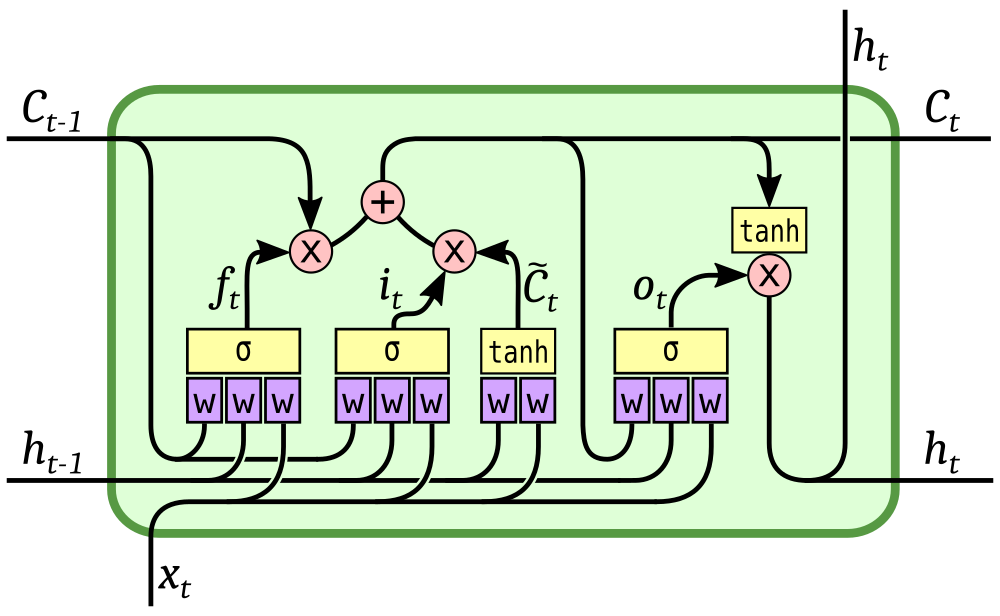
\includegraphics[width=12cm]{lstm}
    \caption{LSTM with peephole connections (Adapted from \cite{rnnplot})}
    \label{Figure:LSTM-structure}
\end{figure}

To address the vanishing/exploding gradient problem, multiple variations of RNN have been proposed. 
Long Short-Term Memory (LSTM) networks are one of the popular architectures \cite{lstm}. 
The structure of LSTM is shown in \fref{Figure:LSTM-structure}. 

The LSTM network introduces three gates to manage the weights of samples in the sequenced data. $f$ is the forget gate, $i$ is input gate, and $o$ is forget gate. 
$\sigma$ is a signoid function that gives a value between 0 and 1, which can act like a switch. 
$\mathbf{h}$ and $\mathbf{c}$ stands for hidden state and cell state. Each carries a memory path to pass down information.  
The equation of each value is given by: 

\begin{gather}
    \mathbf{i} _t=\sigma (\mathbf{w} _{xi}\mathbf{x} _t + \mathbf{w} _{hi}\mathbf{h} _{t-1} + b_i) \notag\\
    f_t=\sigma (\mathbf{w} _{xf}\mathbf{x} _t + \mathbf{w} _{hf}\mathbf{h} _{t-1} + b_f) \notag\\
    \mathbf{o} _t=\sigma (\mathbf{w} _{xo}\mathbf{x} _t + \mathbf{w} _{ho}\mathbf{h} _{t-1} + b_o) \notag\\
    \mathbf{\tilde{c} } _t=\tanh (\mathbf{w} _{xc}\mathbf{x} _t + \mathbf{w} _{hc}\mathbf{h} _{t-1} + b_c) \\
    \mathbf{c} _t=f_t \odot \mathbf{c} _{t-1} + \mathbf{i} _t \odot \mathbf{\tilde{c} } _t \notag\\
    \mathbf{h} _t=\mathbf{o} _t \odot \tanh (\mathbf{c} _t) \notag
\end{gather}

These gates, or rather sigmoid functions, let LSTM choose to ignore a sample if the current sample has been considered as not important. 
Otherwise, the LSTM will discard the information before the sample, and only retain the information of current time $t$. 

In the first version of LSTM, there is no output gate \cite{ribeiro2020exploding}, and the equations looks like this: 

\begin{gather}
    \mathbf{i} _t=\sigma (\mathbf{w} _{xi}\mathbf{x} _t + \mathbf{w} _{hi}\mathbf{h} _{t-1} + b_i) \notag\\
    f_t=\sigma (\mathbf{w} _{xf}\mathbf{x} _t + \mathbf{w} _{hf}\mathbf{h} _{t-1} + b_f) \notag\\
    \mathbf{\tilde{h} } _t=\tanh (\mathbf{w} _{xc}\mathbf{x} _t + \mathbf{w} _{hc}\mathbf{h} _{t-1} + b_c) \\
    \mathbf{h} _t=f_t \odot \mathbf{h} _{t-1} + \mathbf{i} _t \odot \mathbf{\tilde{h} } _t \notag
\end{gather}

It is clearer that in this set of equations, $\mathbf{i}$ controls the weight of short-term memories, and $f$ controls longer memories. 
Those two gates are independent. While training, it can find suitable parameters for $\mathbf{i}$ and $f$, 
which means $\mathbf{i}$ and $f$  will use different $\mathbf{x} _t$ and $\mathbf{h} _{t-1}$ to give different control strategies.

The addition of the output gate and use of $\mathbf{c}$ is to keep the longer memories more effectively. 
$\mathbf{c}$ does not exit the output gate, hence it is not affected if the current output gate is approaching 0. 
Even though the current $f$ is tend to 0, which means $\mathbf{c}_{t-1}$ has been forgotten, $\mathbf{h} _{t-1}$ still contains information about $\mathbf{c}_{t-1}$. 
This allows the long-term memories to pass down through the time sequence. 
